\chapter{Sistemi di Autenticazione}

Per autenticazione si intende il processo che permette di verificare in modo affidabile l'identità di qualcuno (o di qualcosa).\\
Si noti che esistono svariate forme di autenticazione (e.g. una persona può essere riconosciuta dall'aspetto fisico o dalla voce, da una guardia che confronta il viso con la foto nel badge,nel caso degli acquisti on-line, dalle informazioni associate alla carta di credito...); queste possono essere classificate in base 
\begin{itemize}
\item al tipo (persona o computer) di entità coinvolte: autenticazione computer/computer, autenticazione persona/computer, autenticazione persona/persona
\item alle informazioni e al modo in cui l'autenticazione avviene: autenticazione basata su password, autenticazione basata sull'indirizzo, autenticazione crittografica
\end{itemize}

\section{Autenticazione basata su password}
Nel caso di autenticazione basata su password l'identità equivale alla conoscenza della password: chi si deve autenticare invia la propria password, in chiaro, all'entità autenticante, che è in grado di verificare se la password inviata esiste e corrisponde all'utente da cui è stata inviata (\figurename ~\ref{fig:ImgS5}). Ovviamente, le intercettazioni costituiscono la minaccia principale.\\
\begin{figure}[htbp]
	\centering%
	\subfigure%
	{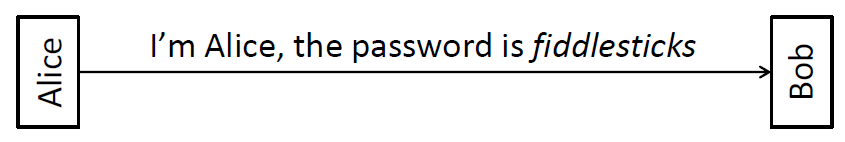
\includegraphics[height=4cm, width=12cm, keepaspectratio]{Immagini/autenticazione/ImgS5.png}}
	\caption{Autenticazione basata su password\label{fig:ImgS5}} 	
\end{figure}
Un'autenticazione che richiede l'inserimento di una password non è detto che ricada nella categoria autenticazione basata su password: se infatti le informazioni inviate risultano cifrate (magari con una chiave derivata dalla password), allora si parlerà di autenticazione crittografica.

\subsubsection{Attacchi alle password}
Gli attacchi alle password possono essere di tipo \textbf{on-line} o \textbf{off-line}.\\ \\
In un attacco on-line si tenta di indovinare la password semplicemente inviandola al sistema autenticante. Per contrastare attacchi di questo tipo si può limitare il numero di tentativi (ad esempio, gli sportelli bancomat ATM ritirano la tessera dopo tre inserimenti errati della password); in alternativa il sistema potrebbe diventare sempre più lento all'aumentare dei tentativi e/o potrebbe insospettirsi e inviare una notifica ad un operatore di sicurezza.\\ \\
In un attacco off-line un avversario può catturare una quantità $X$ derivata dalla password (ad esempio l'hash) con una tecnica nota e poi, prendendosi il tempo che vuole ed usando tutta la potenza di calcolo e di memoria di cui dispone, scegliere password candidata $p$, convertirla nel modo noto in $X_{p}$ e verificare se $X_{p} = X$ (ripetendo tale procedura se l'uguaglianza non sussiste).\\
Un attacco off-line è detto anche dictionary attack perché le password candidate vengono prese da un dizionario (se un avversario può sferrare un attacco off-line, allora è necessario aumentare la grandezza dello spazio cui appartiene il segreto).

\section{Autenticazione basata sull'indirizzo}
Si ha un'autenticazione basata sull'indirizzo se l'identità della sorgente può essere inferita esaminando l'indirizzo di rete dal quale arrivano i pacchetti. L'idea base è che ciascun computer \textit{C} memorizzi delle informazioni che specificano gli account utenti, di altri computer, accreditati ad accedere a \textit{C}: ad esempio, se l'utente Smith del calcolatore residente al nodo di indirizzo \textit{N} ha il permesso di accedere al computer \textit{C} ed eseguire richieste come il log-in e comandi come \textit{copy <source-file> <destination-file>}, se \textit{C} deduce che una richiesta arriva dal nodo \textit{N} e da parte di Smith, allora \textit{C} onorerà tale richiesta.\\ \\
L'autenticazione basata sull'indirizzo è sicura rispetto alle intercettazioni, ma è sottoposta alle seguenti minacce:
\begin{itemize}
\item (R1) se un attaccante ottiene i privilegi su un nodo FOO, oltre a poter accedere alle risorse di tutti gli utenti di FOO, può anche accedere alle risorse di rete di ogni utente con un account su FOO
\item (R2) se un attaccante può impersonare gli indirizzi di rete dei nodi, può accedere a tutte le risorse di rete di tutti gli utenti che hanno un account su qualcuno di tali nodi
\end{itemize}
Dipendentemente dall'ambiente (tipo di rete, sistema operativo e configurazione), l'autenticazione basata sull'indirizzo può essere più o meno sicura rispetto ad inviare password in chiaro: è sicuramente più conveniente/usabile ed è il meccanismo di autenticazione scelto in molti sistemi distribuiti.

\section{Autenticazione crittografica}
I protocolli di autenticazione crittografici possono essere molto più sicuri sia di quelli basati su password (in chiaro) che di quelli basati sull'indirizzo. \\ 
Si noti infatti che in un protocollo di autenticazione crittografico Alice prova la sua identità eseguendo delle operazioni crittografiche su quantità fornite da Bob, queste operazioni dipendono da un'informazione segreta nota solo ad Alice o al più anche a Bob.

\subsection{Intercettazioni e violazioni del server autenticante}
Si consideri un utente, Alice, che deve autenticarsi presso un server remoto Bob per poter fruire dei servizi resi dal server Bob. L'autenticazione deve garantire che nessuno sia in grado di impersonare Alice, anche se riesce ad intercettare i messaggi scambiati tra Alice e Bob, e/o riesce a violare il server Bob e ad accedere in modo non autorizzato al database contenente le informazioni per l'autenticazione.\\
Consideriamo pertanto i seguenti requisiti di sicurezza:
\begin{itemize}
\item protezione rispetto eventuali intercettazioni delle informazioni trasmesse (se un avversario intercetta tali informazioni non deve poter impersonare Alice)
\item protezione rispetto eventuali violazioni del server  e/o accessi in lettura non autorizzati al suo database (se un intruso viola il server Bob e riesce ad accedere al database non deve poter impersonare gli utenti di Bob)
\end{itemize}
Ovviamente, questi requisiti impongono l'adozione di una autenticazione crittografica.\\ 
\subsubsection{Uso di $pwd_{Alice} + PU_{Bob}$}
Proviamo a combinare l'uso della password con tecniche crittografiche a chiave pubblica: la password di Alice è cifrata con la chiave pubblica di Bob e nel database del server Bob la password non è memorizzata in chiaro, ma viene memorizzato il suo digest (\figurename ~\ref{fig:ImgS37}).
\begin{figure}[htbp]
	\centering%
	\subfigure%
	{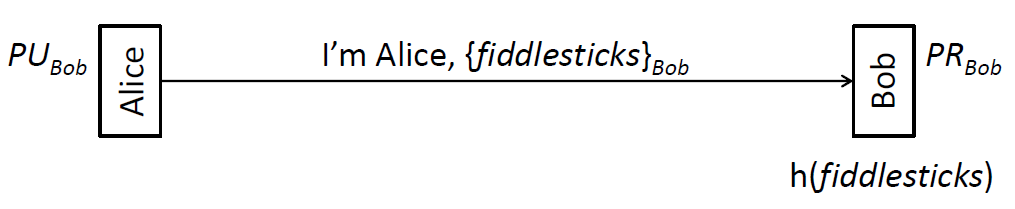
\includegraphics[height=4cm, width=12cm, keepaspectratio]{Immagini/autenticazione/ImgS37.png}}
	\caption{Uso di $pwd_{Alice} + PU_{Bob}$\label{fig:ImgS37}} 	
\end{figure}
Si noti però che con precedente soluzione...
\begin{itemize}
\item il requisito (R1) non è soddisfatto, poichè un impostore potrebbe riusare il messaggio inviato da Alice ed
impersonarla, inoltre potrebbe ottenere la password con un attacco dictionary se non viene applicato lo standard $\symbol{35}PKCS1$
\item (R2) è parzialmente soddisfatto, infatti violando il server Bob si potrebbe ricavare la chiave privata $PR_{Bob}$ (se la password non è robusta un attacco off-line di tipo dictionary permetterebbe di ricavarla)
\end{itemize}
Modifichiamo allora lo schema proposto, come mostrato in \figurename ~\ref{fig:ImgS39}. Siano:
\begin{itemize}
\item random: numero random (tale numero è implicito nello standard $\symbol{35}PKCS1$, perciò se si segue lo standard il numero random può essere omesso)
\item timestamp: intero che codifica l'istante attuale
\item salt: numero random unico associato ad ogni utente
\item f(): una qualche funzione deterministica (può anche essere omessa)
\end{itemize} 
\begin{figure}[htbp]
	\centering%
	\subfigure%
	{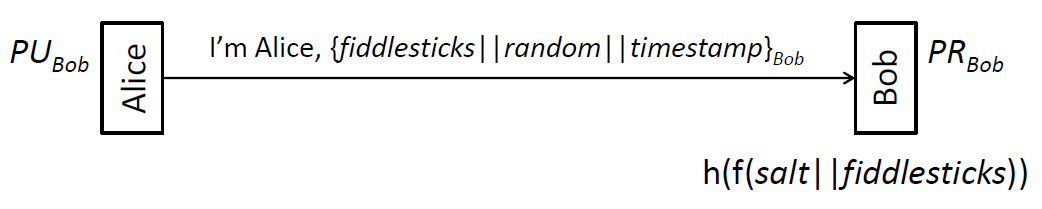
\includegraphics[height=4cm, width=12cm, keepaspectratio]{Immagini/autenticazione/ImgS39.png}}
	\caption{Uso di $pwd_{Alice} + PU_{Bob}$, schema modificato\label{fig:ImgS39}} 	
\end{figure}
Con questa soluzione...
\begin{itemize}
\item (R1) è abbastanza rispettato, infatti la quantità random permette di sventare attacchi di tipo dictionary sulle password cifrate con $PU_{Bob}$ e il timestamp non consente di riciclare messaggi "scaduti" (anche se messaggi molto recenti potrebbero ancora essere riciclati)
\item (R2) è parzialmente soddisfatto, infatti, violando il server Bob si potrebbe ricavare la chiave privata $PR_{Bob}$, ma la presenza del salt rende più difficile l'attacco di tipo dictionary sugli hash memorizzati nel database (anche se l'intruso potrebbe individuare il salt)
\end{itemize}
\subsubsection{Uso di $pwd_{Alice} + segreto condiviso$}
Se non fosse possibile ricorrere alla cifratura a chiave pubblica, si può ricorrere allo schema in \figurename ~\ref{fig:ImgS42}
\begin{figure}[htbp]
	\centering%
	\subfigure%
	{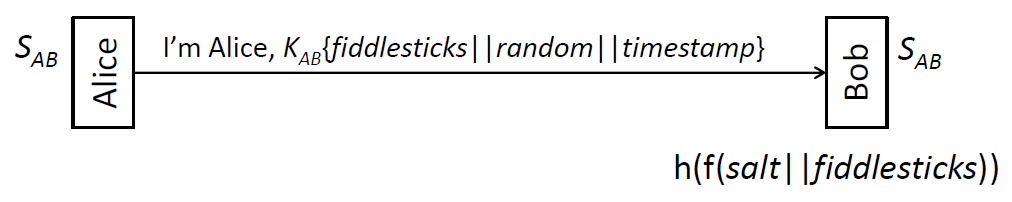
\includegraphics[height=4cm, width=12cm, keepaspectratio]{Immagini/autenticazione/ImgS42.png}}
	\caption{Uso di $pwd_{Alice} + segreto condiviso$\label{fig:ImgS42}} 	
\end{figure}
Si assuma che Alice e Bob condividano un segreto $S_{AB}$ da cui sia possibile ottenere, con una procedura conosciuta, una chiave segreta $K_{AB}$.
Con questa soluzione...
\begin{itemize}
\item (R1) è soddisfatto abbastanza bene
\item (R2) non è soddisfatto, infatti una violazione del server Bob permetterebbe di ottenere il segreto condiviso $S_{AB}$ (che in genere non sarà protetto bene quanto la chiave privata di Bob $PR_{Bob}$, la quale è unica ed è associata al server Bob, quindi può essere protetta in luoghi e modi particolarmente sicuri)
\end{itemize}
\subsubsection{Uso di password in chiaro}
Utilizzando password in chiaro, come nello schema in \figurename ~\ref{fig:ImgS43}...
\begin{figure}[htbp]
	\centering%
	\subfigure%
	{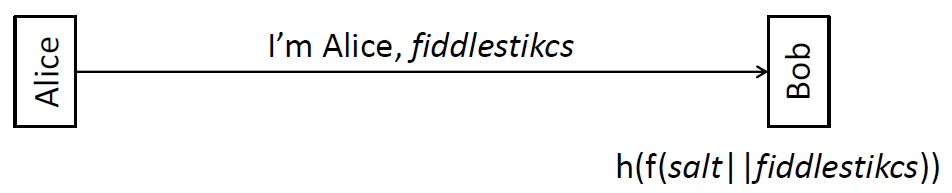
\includegraphics[height=4cm, width=12cm, keepaspectratio]{Immagini/autenticazione/ImgS43.png}}
	\caption{Uso di una password in chiaro\label{fig:ImgS43}} 	
\end{figure}
\begin{itemize}
\item (R1) non è soddisfatto
\item (R2) è soddisfatto abbastanza bene
\end{itemize}
\subsubsection{Uso di chiavi crittografiche}
Nell'ipotesi che Alice (o il suo client) disponga di un qualche tipo di chiave crittografica ($PR_{Alice}$ - una chiave privata - o $K_{AB}$ - una chiave segreta condivisa con Bob, non derivata da password -), si può ricorrere allo schema in \figurename ~\ref{fig:ImgS45}, che non fa uso di password, ma sfrutta le proprietà della firma digitale, soddisfacendo entrambi i requisiti (R1) e (R2).
\begin{figure}[htbp]
	\centering%
	\subfigure%
	{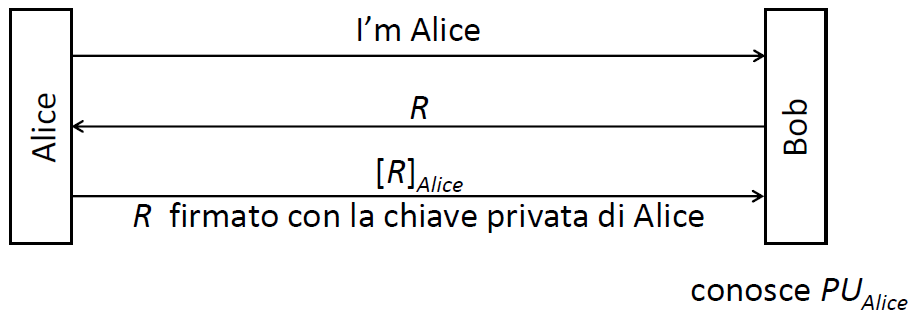
\includegraphics[height=4cm, width=12cm, keepaspectratio]{Immagini/autenticazione/ImgS45.png}}
	\caption{Uso di $PR_{Alice}$\label{fig:ImgS45}} 	
\end{figure}
In alternativa si può applicare lo schema in \figurename ~\ref{fig:ImgS46}, che non fa uso di password e sfrutta una chiave segreta condivisa $K_{AB}$ tra Alice e Bob, soddisfacendo (R1), ma non (R2), perché violando il server
Bob si otterrebbe il segreto $K_{AB}$.
\begin{figure}[htbp]
	\centering%
	\subfigure%
	{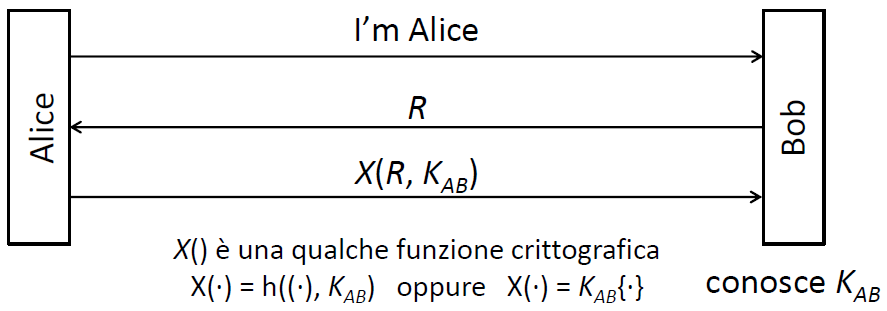
\includegraphics[height=4cm, width=12cm, keepaspectratio]{Immagini/autenticazione/ImgS46.png}}
	\caption{Uso di $K_{AB}$ non derivata da $pwd$\label{fig:ImgS46}} 	
\end{figure}
\subsubsection{Riassumendo}


Se si desidera soddisfare a pieno i requisiti (R1) e (R2) conviene evitare l'uso di password ed è necessario ricorrere alla crittografia a chiave pubblica. Senza la crittografia a chiave pubblica, infatti diventa
molto complicato, se non impossibile, soddisfare contemporaneamente (R1) e (R2), mentre è facile soddisfare o solo (R1) o solo (R2).


\subsection{Intermediari fidati}
\subsubsection{Distribuzione delle chiavi segrete}
Si assuma che la sicurezza di una rete si basi sulla tecnologia a chiave segreta. Se la rete ha \textit{n} nodi, e
ogni computer \textit{c} deve poter autenticare ogni altro nodo, allora \textit{c} deve memorizzare \textit{n – 1} chiavi (una per ogni altro sistema della rete): se un nuovo nodo viene aggiunto alla rete dovrebbero essere generate \textit{n} nuove chiavi per avere una chiave segreta condivisa con tutti gli \textit{n} nodi pre-esistenti. \\
Sarebbe pertanto necessario distribuire tali \textit{n} chiavi in modo sicuro a tutti gli altri nodi della rete, ma tale strategia di gestione delle chiavi può aver senso solo per reti molto piccole (\figurename ~\ref{fig:ImgS50}). 
\begin{figure}[htbp]
	\centering%
	\subfigure%
	{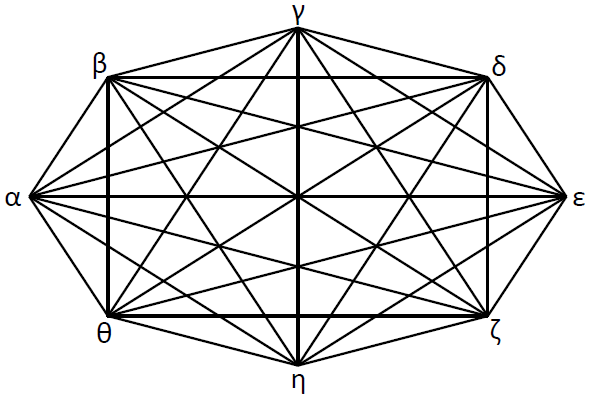
\includegraphics[height=4cm, width=12cm, keepaspectratio]{Immagini/autenticazione/ImgS50.png}}
	\caption{Distribuzione delle chiavi\label{fig:ImgS50}} 	
\end{figure}
Un centro di distribuzione delle chiavi, \textbf{K}ey \textbf{D}istribution \textbf{C}enter (KDC), agevola la gestione/distribuzione delle chiavi segrete: conosce le chiavi di tutti i nodi e se un nuovo nodo si aggiunge alla rete, sola una chiave segreta, condivisa tra quel nodo e il KDC, deve essere generata (\figurename ~\ref{fig:ImgS52}). 
\begin{figure}[htbp]
	\centering%
	\subfigure%
	{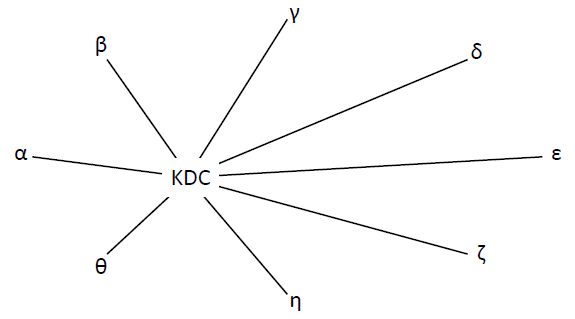
\includegraphics[height=4cm, width=12cm, keepaspectratio]{Immagini/autenticazione/ImgS52.png}}
	\caption{Distribuzione delle chiavi con KDC\label{fig:ImgS52}} 	
\end{figure}

\subsubsection{Centri di distribuzione delle chiavi}
Se un nodo $\alpha$ deve comunicare con un nodo $\beta$, $\alpha$ comunica con il KDC in modo sicuro, e usando la loro chiave segreta condivisa $K_{\alpha KDC}$ gli chiede di inviargli una chiave per comunicare con $\beta$; il KDC autentica $\alpha$, sceglie un numero random $ R_{\alpha\beta} $ da usare come chiave segreta condivisa tra $\alpha$ e $\beta$; cifra $ R_{\alpha\beta} $ con la chiave segreta $K_{\beta KDC}$ che condivide con $\beta$, e trasmette a $\beta$ $ R_{\alpha\beta} $ cifrata insieme alle istruzioni che $\beta$ deve usare per comunicare con $\alpha$ (in genere, il KDC non trasmette direttamente $ R_{\alpha\beta} $ cifrato a $\beta$, per confinare il suo intervento all'interazione con un solo nodo e prevenire attacchi di DoS, ma lo invia ad $\alpha$ che poi lo inoltrerà a $\beta$:
il messaggio cifrato per $\beta$ che il KDC invia ad $\alpha$, e che $\alpha$ dovrà inoltrare a $\beta$ e detto \textbf{ticket}, che, oltre a contenere $ R_{\alpha\beta} $ contiene altre informazioni utili, come data di scadenza, nome del nodo $\alpha$, ecc.). \\ \\
I KDC semplificano la distribuzione delle chiavi: quando un nuovo utente deve essere aggiunto alla rete, o quando si sospetta che una chiave d'utente sia stata compromessa, c'è un singolo punto della rete, il KDC, la cui configurazione deve essere aggiornata. L'alternativa al KDC è installare le informazioni di un utente in ciascun server ove potrebbe accedere. \\
L'uso dei KDC comporta però i seguenti svantaggi: 
\begin{itemize}
\item contiene tutte le informazioni per impersonare un utente ad un qualsiasi altro utente, perciò, se compromesso, tutte le risorse di rete risultano vulnerabili
\item è un "single point of failure", quindi in caso di guasto nessuno può iniziare una comunicazione con nuovi utenti (le chiavi precedentemente distribuite continuano a funzionare)
\item è possibile avere più KDC (KDC multipli) con lo stesso database di chiavi, ma ciò comporta una maggior complessità di gestione, costi extra per le macchine e per la replicazione dei protocolli e maggiori vulnerabilità (è necessario proteggere più target da eventuali attacchi)
\item può costituire un collo di bottiglia (in questa caso, avere più di un KDC può alleviare tale problema)
\end{itemize}  

\subsubsection{Autorità di certificazione}
La distribuzione delle chiavi è più facile con la crittografia a chiave pubblica: ogni nodo deve custodire soltanto la propria chiave privata e tutte le chiavi pubbliche possono essere accessibili in un unico punto. \\
Anche in questo caso continuano ad esserci dei problemi: chi garantisce che le chiavi pubbliche disponibili in un dato punto siano corrette (corrispondano realmente alle entità a cui sono associate)? \\
Per evitare la falsificazione delle chiavi pubbliche si ricorre alle Autorità di Certificazione. \\
Una Autorità di Certificazione, \textbf{C}ertification \textbf{A}uthority CA, è un intermediario fidato che genera i certificati, cioè dei messaggi firmati dalla CA contenenti il nome, la chiave pubblica ed altre informazioni di uno specifico nodo. Tutti i nodi dovranno essere pre-configurati con la chiave pubblica della CA, in modo tale da poter verificare la sua firma sui certificati rilasciati: si tratta dell'unica (in questo specifico esempio) chiave pubblica che devono conoscere a priori. \\ \\
Lo \textbf{standard X.509} per le infrastrutture a chiave pubblica ha definito il formato standard di un certificato. \\
Un \textbf{certificato} contiene:
\begin{itemize}
\item il nome utente (persone fisica, organizzazione, server, applicazione, …)
\item la chiave pubblica dell'utente
\item la data di scadenza
\item un numero seriale
\item la firma, della CA che lo ha emesso, dell'intero contenuto del certificato
\end{itemize}
I certificati possono essere memorizzati nel luogo ritenuto più conveniente (e.g. in un directory service), oppure
ciascun nodo può memorizzare i certificati d'interesse e trasmetterli durante lo "scambio di autenticazione". 
In un certo senso le CA sono la controparte dei KDC nelle infrastrutture a chiave pubblica: CA e KDC costituiscono l'intermediario fidato la cui compromissione può arrecare seri danni all'integrità della rete. \\ \\
Si noti che non è necessario che la CA sia on-line: può risiedere in una stanza fisicamente ben protetta (magari con una guardia) e si può limitare l'accesso alla CA ad una sola persona di grande fiducia. Questa persona, interagendo con la CA, genera il certificato di un dato utente, lo memorizza su un qualche supporto di memoria esterna che può consegnare "a mano" al diretto interessato. Se la CA non è on-line, nessun potenziale intruso può accedervi per ottenere informazioni utili, non deve implementare protocolli di rete che richiedono elevata efficienza computazionale, quindi può essere implementata da un dispositivo estremamente semplice e pertanto molto più sicuro.\\ 
Se la CA dovesse "crashare", la rete continuerebbe a funzionare, ma non sarebbe possibile aggiungere nuovi utenti o
revocare certificati compromessi o di utenti sospetti, pertanto non è essenziale avere CA multiple. \\
I certificati sono poco sensibili ad eventuali attacchi: se memorizzati in modo conveniente, ma potenzialmente
insicuro (ad es. in un servizio di directory), un sabotatore può cancellare i certificati, impedendo l'accesso ai corrispondenti nodi della rete (attacco DOS) ma non può creare dei certificati fasulli o modificarli in qualche modo se non dispone della chiave privata della CA.\\
Una CA compromessa non può decifrare le conversazioni tra due nodi (reali) da lei serviti (mentre un KDC compromesso può decifrare tutte le conversazioni tra coppie di nodi da lui serviti), pertanto una CA compromessa può ingannare un utente, diciamo Alice, inviandogli una falsa chiave pubblica di Bob e riuscire ad impersonare Bob in una comunicazione con Alice, ma non può decifrare una comunicazione tra la vera Alice e il vero Bob: quindi la compromissione di una CA rimane un fatto molto grave, ma non quanto la compromissione di un KDC. \\ \\
Le CA presentano comunque il seguente svantaggio rispetto i KDC: \\
Supponiamo che Fred offra dei servizi di hosting per conto dell'azienda X SpA; la società X SpA fornisce a Fred un certificato (rilasciato a favore della X SpA) necessario ad autenticare il server, pertanto Fred conosce la chiave privata della chiave pubblica certificata. Supponiamo inoltre che a causa di un contrasto con Fred, la X SpA decida di interrompere il rapporto di lavoro; se il certificato è ancora valido Fred può continuare a rendere dei servizi per conto della X SpA, magari anche danneggiandola. Per la X SpA sarebbe importante informare gli utenti di non accettare il certificato generato per Fred e ancora in corso di validità. \\
Con i KDC tale problema è di facile soluzione: basta rimuovere $K_{Fred}$ dal KDC.\\ 
Ovviamente si ha un problema analogo anche quando viene smarrita, o peggio rubata, la chiave privata associata alla chiave pubblica certificata.\\
Nel caso delle CA non è facile estromettere qualcuno che detiene una chiave privata la cui chiave pubblica è certificata (si noti che potrebbe essere molto rischioso attendere la scadenza naturale del certificato); in queste situazioni conviene revocare il certificato: si revoca un certificato quando, a partire da un certo momento, non devono essere più considerate valide le firme generate con la chiave privata abbinata alla chiave pubblica contenuta nel certificato. \\ \\
La \textbf{revoca} di un certificato si attua inserendo un riferimento al certificato all'interno di una lista di revoca (\textbf{C}ertificate \textbf{R}evocation \textbf{L}ist CRL), che elenca i numeri seriali di certificati da non onorare. Ogni CA pubblica periodicamente una nuova CRL che contiene tutti i certificati revocati e non scaduti.\\
Un certificato è valido se:
\begin{itemize}
\item la firma della CA è valida,
\item non è scaduto
\item non è inserito nella CRL più recente della CA che lo ha emesso
\item la CRL ha una data e ora di emissione
\end{itemize}
Se un'applicazione vuole assicurarsi che nessuno dei certificati che onora sia stato revocato entro un'ora prima
della verifica, allora deve essere trascorsa al più un ora dal momento in cui la CRL, consultata da tale applicazione, è stata emessa; quindi, in questo caso, una nuova CRL deve essere pubblicata con una cadenza di un'ora.\\
Un intruso potrebbe cancellare l'ultima CRL, in tal caso le applicazioni configurate per consultare esclusivamente CRL pubblicate nell'ultima ora si rifiuteranno di onorare tutti i certificati, ma l'intruso non può impersonare un utente valido distruggendo la CRL o sovrascrivendola con una CRL più vecchia.\\
Lo standard X.509 ha definito anche il formato delle CRL, in base al quale una CRL deve includere:
\begin{itemize}
\item una lista di numeri seriali di certificati revocati e non scaduti
\item e una data e ora di emissione della CRL
\item la firma dell'intera lista con la chiave privata della CA
\end{itemize}
\paragraph{Problema}
Supponendo che Bob sia un'applicazione che deve autenticare l'utente Alice, illustrare un possibile protocollo di
autenticazione a chiave pubblica, che includa una verifica dell'appartenenza della chiave pubblica all'utente Alice.
\\ \\
Chiaramente Bob ha bisogno del certificato di Alice, \textit{$Cert_{Alice}$}, e di una CRL recente: Bob può ottenerli da un servizio di directory, oppure Alice li trasmette a Bob. 
\begin{figure}[htbp]
	\centering%
	\subfigure%
	{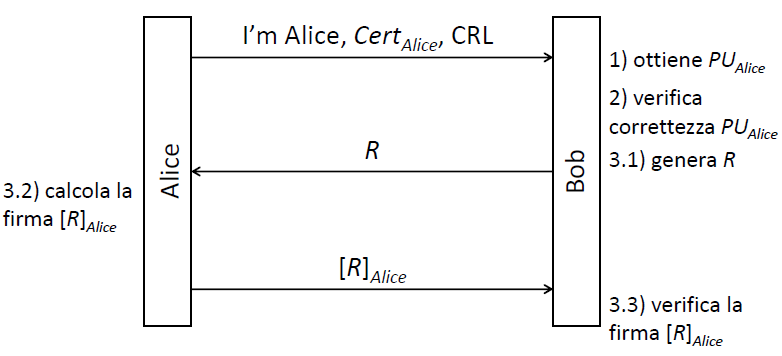
\includegraphics[height=4cm, width=12cm, keepaspectratio]{Immagini/autenticazione/ImgS76.png}}
	\caption{Possibile soluzione per l'autenticazione a chiave pubblica\label{fig:ImgS76}} 	
\end{figure}
In riferimento alla \figurename ~\ref{fig:ImgS76}, una possibile soluzione è:
\begin{itemize}
\item Bob recupera il certificato di Alice \textit{$Cert_{Alice}$} e una CRL recente
\item Consultando il certificato \textit{$Cert_{Alice}$} individua la chiave pubblica di Alice \textit{$PU_{Alice}$}
\item Verifica la correttezza di \textit{$PU_{Alice}$} come segue:
\begin{itemize}
\item se il certificato \textit{$Cert_{Alice}$} è correttamente firmato dalla CA che lo ha emesso e non è scaduto, e
la CRL è correttamente firmata dalla CA ed è sufficientemente recente e non contiene il certificato \textit{$Cert_{Alice}$}, allora Bob conclude che \textit{$PU_{Alice}$} è corretta (quindi è quella nel certificato)
\end{itemize}
\item Bob ed Alice iniziano uno scambio di messaggi seguendo uno schema di autenticazione a chiave pubblica, ad esempio:
\begin{itemize}
\item Bob invia una sfida \textit{R} ad Alice
\item Alice firma \textit{R} con la propria chiave privata ed invia [\textit{R}]\textit{$_{Alice}$} a Bob
\item Bob verifica la firma di Alice ed in caso affermativo autentica Alice
\end{itemize}
\end{itemize}

\section{Protocolli a sfida e risposta unidirezionali ("login only")}
Nel seguito si userà la seguente notazione:
\begin{itemize}
\item $R$: sfida, numero casuale e non prevedibile
\item $K_{Alice-Bob}\lbrace R\rbrace$: cifratura di $R$ con un algoritmo a chiave segreta (DES, AES), dove $K_{Alice-Bob}$ è la chiave di cifratura
\item $h(K_{Alice-Bob}, R)$: hash di $R$ dipendente dal segreto $K_{Alice-Bob}$ (e.g. la sfida $R$ può essere concatenata con $K_{Alice-Bob}$)
\item $f(K_{Alice-Bob}, R)$: quantità ottenuta applicando ad $R$ una trasformazione crittografica dipendente dal segreto (i.e. $f(K_{Alice-Bob}, R)$ può essere sia $K_{Alice-Bob}\lbrace R\rbrace$ sia $h(K_{Alice-Bob}, R)$)
\end{itemize}
\subsubsection{(P1) Protocollo 1 – Chiave segreta unidirezionale}
Si consideri il protocollo di tipo "login only", in \figurename ~\ref{fig:ImgS11bis}
\begin{figure}[htbp]
	\centering%
	\subfigure%
	{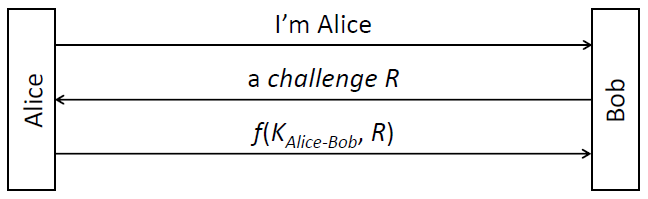
\includegraphics[height=4cm, width=12cm, keepaspectratio]{Immagini/autenticazione/ImgS11bis.png}}
	\caption{Bob autentica Alice sfruttando un segreto condiviso $K_{Alice-Bob}$\label{fig:ImgS11bis}} 	
\end{figure}
Tale protocollo rappresenta un notevole passo in avanti rispetto a spedire la password in chiaro, infatti uno spione non può impersonare Alice "ascoltando" lo scambio perché la sfida $R$ cambia di volta in volta in modo non prevedibile.\\
Si noti che il protocollo (P1) presenta le seguenti debolezze:
\begin{itemize}
\item Non c'è mutua autenticazione: Bob autentica Alice, ma non viceversa. Se Trudy può ricevere i pacchetti inviati all'indirizzo di rete di Bob, e può rispondere con l'indirizzo di rete di Bob (o attraverso altri mezzi convince Alice che il suo indirizzo e quello di Bob), allora Alice sarà ingannata e crederà che Trudy sia Bob (si noti che Trudy non ha bisogno di conoscere il segreto condiviso $K_{Alice-Bob}$ per impersonare Bob, deve solo limitarsi ad inviare ad Alice una qualsiasi vecchia sfida $R$ e ignorare la sua risposta)
\item Se non è prevista alcuna protezione della confidenzialità del resto della conversazione, allora Trudy può dirottare la conversazione dopo lo scambio iniziale, assumendo che sia in grado di generare pacchetti aventi per source address l'indirizzo di Alice (IP spoofing). Potrebbe anche essere utile, ma non essenziale, per Trudy, poter ricevere pacchetti indirizzati ad Alice
\item Se il segreto condiviso $K_{Alice-Bob}$ fosse derivato da una password, allora conoscendo $R$, $f(K_{Alice-Bob}, R)$ e l'algoritmo per ottenere la chiave dalla password, un intercettatore potrebbe sferrare un attacco off-line sulla password: scegliendo una parola $w$, quale password candidata, calcolando la relativa chiave segreta $K_{w}$ e verificando se $f(K_{w}, R) = f(K_{Alice-Bob}, R)$ (in caso negativo ritenta)
\item Qualcuno che acceda (in lettura) al server Bob potrebbe ottenere $K_{Alice-Bob}$: ciò è particolarmente rischioso se $K_{Alice-Bob}$ fosse derivata da una password, e le password fossero memorizzate in un database di
Bob. Proteggere il database implica proteggere tutti i suoi backup impedendone l'accesso fisico o cifrando il contenuto e proteggendo in qualche modo la chiave di cifratura.
\end{itemize}
Nonostante i precedenti svantaggi, se le risorse per aumentare la sicurezza sono molto limitate, il protocollo (P1) costituisce un'alternativa molto più sicura rispetto ad inviare password in chiaro anche se $K_{Alice-Bob}$ viene derivata dalla password.
\subsubsection{(P2) Protocollo 2}
Una piccola variante del protocollo (P1) è riportata in \figurename ~\ref{fig:ImgS17bis}
\begin{figure}[htbp]
	\centering%
	\subfigure%
	{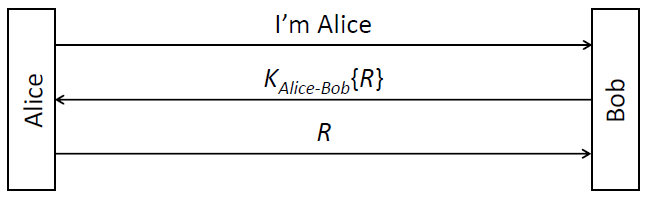
\includegraphics[height=4cm, width=12cm, keepaspectratio]{Immagini/autenticazione/ImgS17bis.png}}
	\caption{Bob autentica Alice sfruttando una chiave segreta condivisa $K_{Alice-Bob}$\label{fig:ImgS17bis}} 	
\end{figure}
Bob sceglie una sfida random $R$, la cifra, e trasmette il risultato; Alice decifra la quantità ricevuta, usando $K_{Alice-Bob}$ per ottenere $R$, ed invia $R$ a Bob.\\
Si noti che (P2) richiede l'uso di operazioni crittografiche invertibili, mentre (P1) può essere implementato usando solo algoritmi di hash (che in genere offrono migliori prestazioni e maggior portabilità). \\
Si noti anche che se $K_{Alice-Bob}$ è derivata da una password (ed è pertanto vulnerabile ad attacchi dictionary) e se inoltre $R$ è una quantità riconoscibile (e.g. 32 bit random + 32 bit nulli di padding), allora Trudy può eseguire un attacco dictionary senza dover essere in grado di intercettare i messaggi (cosa non sempre facile). Ovviamente, se Trudy può intercettare i messaggi scambiati tra le parti, allora può eseguire un attacco dictionary in entrambi i
protocolli (P1) e (P2).\\
Si noti infine che se $R$ e una quantità riconoscibile con tempo di vita limitato (e.g. $R = random||timestamp$), allora anche Alice può autenticare Bob (autenticazione mutua); infatti, soltanto chi conosce $K_{Alice-Bob}$ può generare $K_{Alice-Bob}\lbrace R\rbrace = K_{Alice-Bob\lbrace random||timestamp\rbrace}$, perciò è essenziale che $R$ abbia una durata temporale molto limitata per evitare che $K_{Alice-Bob}\lbrace R\rbrace$ possa essere riciclato da un falso Bob.
\subsubsection{(P3) Protocollo 3}
Quella in \figurename ~\ref{fig:ImgS20bis} è un'altra variante di (P1) che utilizza un timestamp invece di una sfida random $R$, perciò è sufficiente un solo messaggio per l'handshake.
\begin{figure}[htbp]
	\centering%
	\subfigure%
	{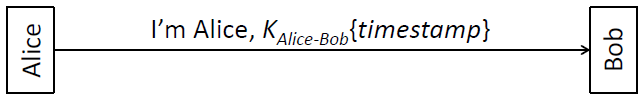
\includegraphics[height=4cm, width=12cm, keepaspectratio]{Immagini/autenticazione/ImgS20bis.png}}
	\caption{Bob autentica Alice sfruttando la sincronizzazione degli orologi e un segreto condiviso $K_{Alice-Bob}$\label{fig:ImgS20bis}} 	
\end{figure}
Alice cifra l'istante temporale corrente, Bob decifra il risultato e si assicura che sia un istante temporale circa uguale a quello fornito dal suo orologio, perciò è necessario che gli orologi di Alice e Bob siano ragionevolmente ben sincronizzati.\\
Il protocollo (P3) può facilmente rimpiazzare un protocollo non crittografico in cui la password è inviata in chiaro, infatti non è necessario aggiungere lo scambio di ulteriori messaggi.\\
(P3) è più efficiente di (P1), infatti, oltre a risparmiare due messaggi, il server Bob non deve mantenere alcuno stato volatile (ad esempio $R$) riguardo Alice (assumendosi qualche rischio), inoltre (P3) può essere aggiunto ad un qualsiasi protocollo di tipo request/response (come l'HTTP) ottenendo un'autenticazione mutua, basta che Bob invii ad Alice una risposta dipendente in modo opportuno dal suo timestamp originario (si vedrà in seguito).
Si noti che qualcuno potrebbe impersonare Alice intercettando e riusando $K_{Alice-Bob}\lbrace timestamp\rbrace$; tale attacco va però eseguito subito dopo aver intercettato $K_{Alice-Bob}\lbrace timestamp\rbrace$, infatti il timestamp generato dal server Bob non deve essere troppo diverso da quello di Alice (un modo per sventare tale minaccia è memorizzare nel server Bob tutti i timestamp ricevuti e non ancora scaduti). \\
Si ha un'altra potenziale debolezza se Alice usa lo stesso segreto $K_{Alice-Bob}$ con più server distinti, infatti un intercettatore che opera in modo veloce può ottenere la quantità $K_{Alice-Bob}\lbrace timestamp\rbrace$ trasmessa ad un server per impersonare Alice con un altro server; tuttavia, tale minaccia è sventabile concatenando il nome del
server con il timestamp, i.e. al posto di $K_{Alice-Bob}\lbrace timestamp\rbrace$ va inviato $K_{Alice-Bob}\lbrace "Bob"||timestamp\rbrace$ (ma (P3) rimane vulnerabile ad eventuali modifiche all'orologio di sistema del server Bob, a causa delle quali timestamp scaduti possono essere riusati). Alla luce di questo, se la sicurezza dipende dall'ora, allora la configurazione dell'ora richiederà un handshake sicuro: un handshake basato sull'istante corrente potrebbe fallire se i due orologi non sono sincronizzati, quindi è necessaria un'autenticazione basata su un handshake di
tipo challenge/response per la sincronizzazione degli orologi.\\
Si ricordi che in (P1), calcolare f(KAlice-Bob, R) voleva dire calcolare $K_{Alice-Bob}\lbrace R\rbrace$ oppure calcolare l'hash $h(R||K_{Alice-Bob})$; ciò continua a valere nel caso del (P3), ma con piccole complicazioni aggiuntive se si usa l'hash: in particolare Bob deve eseguire un certo numero di tentativi per verificare
che $h(timestamp||K_{Alice-Bob})$ sia stato generato da Alice (e.g. se si accettano 10 minuti di differenza tra i due orologi e il timestamp è espresso in minuti, allora 20 tentativi sono sufficienti, ma per timestamp in microsecondi sono necessari più di un miliardo di tentativi!).

\subsubsection{(P4) Protocollo 4}
Assumendo che si voglia utilizzare un timestamp in microsecondi e una funzione di hash anziché una funzione crittografica invertibile, una possibile soluzione è che Alice trasmetta anche il timestamp non cifrato (\figurename ~\ref{fig:ImgS25bis}).
\begin{figure}[htbp]
	\centering%
	\subfigure%
	{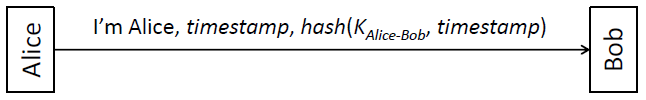
\includegraphics[height=4cm, width=12cm, keepaspectratio]{Immagini/autenticazione/ImgS25bis.png}}
	\caption{Bob autentica Alice calcolando l’hash di un timestamp ad alta risoluzione e sfruttando e un segreto condiviso $K_{Alice-Bob}$\label{fig:ImgS25bis}} 	
\end{figure}
\subsubsection{(P5) Protocollo 5 – Chiave pubblica unidirezionale}
Tutti i precedenti protocolli, a chiave segreta, consentono a Trudy di impersonare Alice se può leggere il database del server; utilizzando la tecnologia a chiave pubblica questa vulnerabilità può essere evitata (\figurename ~\ref{fig:ImgS26bis}).
\begin{figure}[htbp]
	\centering%
	\subfigure%
	{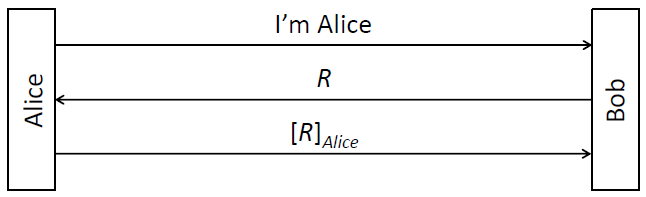
\includegraphics[height=4cm, width=12cm, keepaspectratio]{Immagini/autenticazione/ImgS26bis.png}}
	\caption{Bob autentica Alice verificando la sua firma digitale}\label{fig:ImgS26bis} 	
\end{figure}
Si noti che $[R]_{Alice}$ è $R$ firmato da Alice, cioè cifrato con la sua chiave privata $PR_{Alice}$; Bob verifica la firma $[R]_{Alice}$ usando la chiave pubblica di Alice $PU_{Alice}$ ed accetta il login se il risultato è $R$. Il vantaggio di questo protocollo è che il database di Bob non è più vulnerabile agli accessi in lettura non
autorizzati, tuttavia il database di Bob va comunque protetto da modifiche non autorizzate, ma non da accessi non
autorizzati in lettura (infatti qualcuno potrebbe modificare la chiave pubblica di Alice!).
\subsubsection{(P6) Protocollo 6}
Una variante al (P5) è quella riportata in \figurename ~\ref{fig:ImgS28bis}:
\begin{figure}[htbp]
	\centering%
	\subfigure%
	{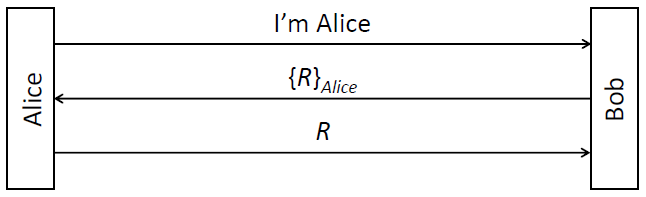
\includegraphics[height=4cm, width=12cm, keepaspectratio]{Immagini/autenticazione/ImgS28bis.png}}
	\caption{Bob autentica Alice se lei può decifrare un messaggio cifrato con la sua chiave pubblica}\label{fig:ImgS28bis} 	
\end{figure}
In questo schema Bob sceglie $R$ e la cifra con $PU_{Alice}$, Alice dimostra di conoscere $PR_{Alice}$ decifrando $\lbrace R\rbrace_{Alice}$ e recuperando $R$.\\
Un problema di questa variante è che molte tecnologie a chiave pubblica (si pensi a DSS) permettono solo di firmare
e non di decifrare.

\section{Protocolli a sfida e risposta, mutua autenticazione} \label{par:aut_prot_mut_aut}
\subsubsection{(P7) Protocollo 7 – Mutua autenticazione a chiave segreta}
Se si desidera autenticare reciprocamente ambo le parti è sufficiente eseguire uno scambio di autenticazione in
entrambe le direzioni (\figurename ~\ref{fig:ImgS35bis}).
\begin{figure}[htbp]
	\centering%
	\subfigure%
	{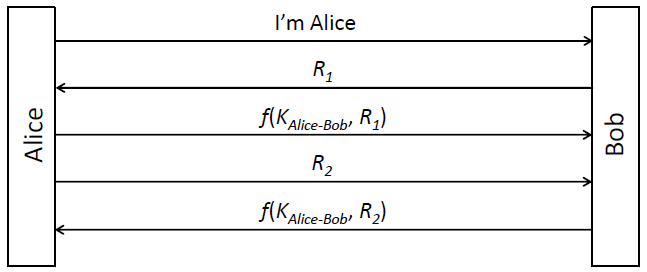
\includegraphics[height=4cm, width=12cm, keepaspectratio]{Immagini/autenticazione/ImgS35bis.png}}
	\caption{Mutua autenticazione basata su un segreto condiviso $K_{Alice-Bob}$}\label{fig:ImgS35bis} 	
\end{figure}
\subsubsection{(P8) Protocollo 8 - Mutua autenticazione a chiave segreta}
Il protocollo (P7) richiede lo scambio di cinque messaggi complessivi, quindi è poco efficiente. Sembra immediato poter ridurre a tre il numero di messaggi caricando in ogni messaggio più informazioni (\figurename ~\ref{fig:ImgS36bis}).
\begin{figure}[htbp]
	\centering%
	\subfigure%
	{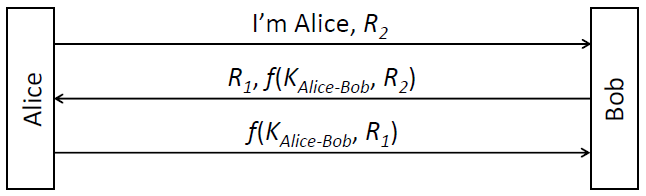
\includegraphics[height=4cm, width=12cm, keepaspectratio]{Immagini/autenticazione/ImgS36bis.png}}
	\caption{Mutua autenticazione ottimizzata basata su un segreto condiviso $K_{Alice-Bob}$}\label{fig:ImgS36bis} 	
\end{figure}
Il protocollo (P8), più compatto del (P7), è però vulnerabile ad un attacco di tipo \textbf{reflection} (\figurename ~\ref{fig:ImgS39bis}). \\
Si supponga che Trudy voglia impersonare Alice: Trudy inizia il protocollo (P8), ma quando riceve la sfida di Bob non può proseguire non potendo cifrare $R_{1}$. Tuttavia, Trudy può interrompere temporaneamente la sessione corrente e può iniziarne una nuova usando $R_{1}$ quale sfida per Bob. A questo punto comunque Trudy non può completare la seconda sessione poiché non può cifrare $R_{3}$, ma ora conosce $f(K_{Alice-Bob},R_{1})$ e può completare la prima sessione rimasta appesa.
\begin{figure}[htbp]
	\centering%
	\subfigure%
	{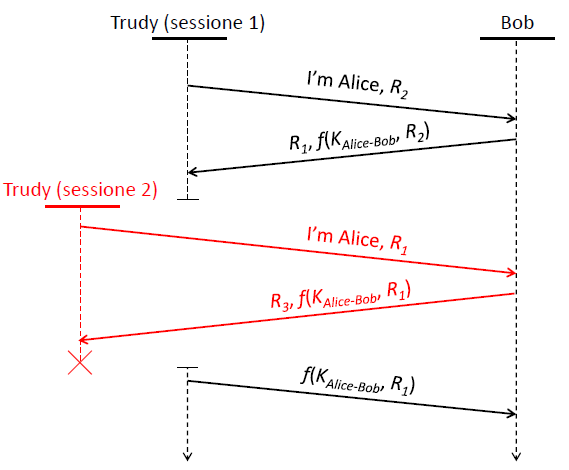
\includegraphics[height=6.5cm, width=12cm, keepaspectratio]{Immagini/autenticazione/ImgS39bis.png}}
	\caption{Attacco di tipo reflection}\label{fig:ImgS39bis} 	
\end{figure}
Un attacco di tipo reflection è facile da sferrare se è possibile aprire simultaneamente più connessioni con lo
stesso server, così infatti ci sarebbero più server che condividono uno stesso segreto con Alice.\\
Tale attacco può essere sventato con un po' di attenzione e comprendendo bene la debolezza che sfrutta, ovvero che Alice e Bob sono perfettamente interscambiabili visto che la risposta ad una stessa sfida è identica.\\
Alla luce di questo, l'idea è quella di differenziare, in qualche modo, la risposta di Alice e quella di Bob ad una stessa sfida seguono alcune possibili soluzioni:
\begin{itemize}
\item Usare chiavi differenti: una possibilità è che Alice e Bob condividano due chiavi completamente differenti, $K_{AAB}$ e $K_{ABB}$, e che Alice cifri con $K_{AAB}$, mentre Bob cifri con $K_{ABB}$; in alternativa, una delle chiavi può essere derivata dall'altra (e.g. $K_{ABB} = -K_{AAB}$ oppure $K_{ABB} = K_{AAB} + 1$ oppure $K_{ABB} = K_{AAB} \oplus F0F0F0F0F0F0F0F0_{16}$)
\item Usare sfide strutturalmente differenti: garantire cioè che la sfida dell'iniziatore abbia una struttura diversa da quella di chi risponde (e.g. l'iniziatore potrebbe usare un numero dispari mentre il risponditore un numero pari)
\item Usare risposte dipendenti dal risponditore: cioè la risposta non deve consistere nella cifratura della sola sfida, ma viene aggiunta un'informazione associata in modo univoco al risponditore (e.g. la risposta ad una sfida $R$ non è semplicemente $f(K, R)$ ma $f(K, R||"nome-id-risponditore"$)
\end{itemize}
Si noti che il protocollo (P7) non è vulnerabile ad un attacco di tipo reflection, poiché segue un altro importante
principi generale, i.e. idealmente, l'iniziatore dovrebbe essere il primo a provare la sua identità.
\subsubsection{(P9) Protocollo 9}
Aggiungendo un messaggio al protocollo (P8) è possibile renderlo molto più robusto ad attacchi off-line sulla password (\figurename ~\ref{fig:ImgS45bis}).
\begin{figure}[htbp]
	\centering%
	\subfigure%
	{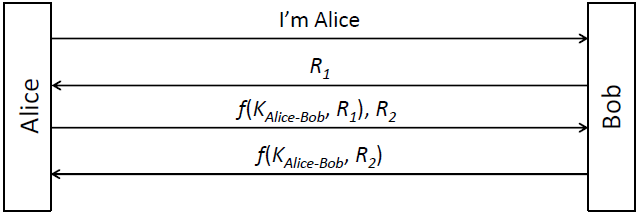
\includegraphics[height=4cm, width=12cm, keepaspectratio]{Immagini/autenticazione/ImgS45bis.png}}
	\caption{Mutua autenticazione parzialmente ottimizzata basata su un segreto condiviso $K_{Alice-Bob}$}\label{fig:ImgS45bis} 	
\end{figure}
Si noti che il nuovo protocollo è chiaramente meno efficiente. Si noti anche che ora Trudy non può più effettuare un attacco off-line sulla password semplicemente spacciandosi per Alice, i.e. senza dover intercettare i messaggi; tuttavia, impersonando l'indirizzo di Bob può tentare di ingannare Alice facendogli stabilire una connessione con lei
(tale vulnerabilità non va ignorata, ma è comunque molto più difficile da sfruttare per un attaccante).
\subsubsection{(P10) Protocollo 10 – Mutua autenticazione a chiave pubblica}
Assumendo che Alice e Bob conoscano ognuno la chiave pubblica dell'altro, utilizzando la tecnologia a chiave pubblica, possono autenticarsi reciprocamente scambiandosi tre messaggi (\figurename ~\ref{fig:ImgS47bis}).
\begin{figure}[htbp]
	\centering%
	\subfigure%
	{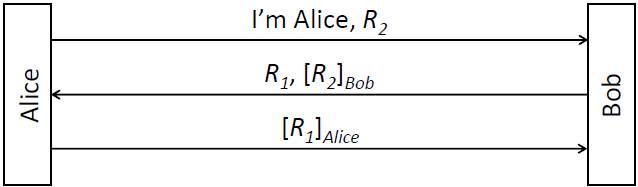
\includegraphics[height=4cm, width=12cm, keepaspectratio]{Immagini/autenticazione/ImgS48bis.png}}
	\caption{Mutua autenticazione a chiave pubblica (basata sulla cifratura/decifratura)}\label{fig:ImgS47bis} 	
\end{figure}
\subsubsection{(P11) Protocollo 11 – Mutua autenticazione a chiave pubblica/timestamp}
Una variante del protocollo (P10) e che fa uso della firma digitale è riportata in \figurename ~\ref{fig:ImgS48bis}:
\begin{figure}[htbp]
	\centering%
	\subfigure%
	{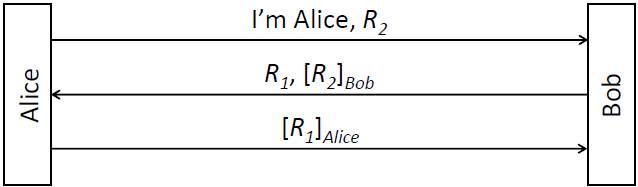
\includegraphics[height=4cm, width=12cm, keepaspectratio]{Immagini/autenticazione/ImgS48bis.png}}
	\caption{Mutua autenticazione a chiave pubblica (basata sulla firma digitale)}\label{fig:ImgS48bis} 	
\end{figure}
Utilizzando dei timestamp, anziché sfide random, è possibile ottenere un protocollo di mutua autenticazione di due soli messaggi: tale soluzione è molto utile e può essere facilmente aggiunta ai protocolli a richiesta/risposta (HTTP) senza dover aggiungere un ulteriore messaggio (\figurename ~\ref{fig:ImgS53bis}).
\begin{figure}[htbp]
	\centering%
	\subfigure%
	{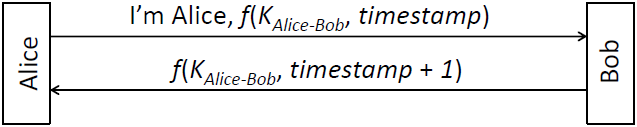
\includegraphics[height=4cm, width=12cm, keepaspectratio]{Immagini/autenticazione/ImgS53bis.png}}
	\caption{Mutua autenticazione basata sulla sincronizzazione degli orologi e su un segreto condiviso $K_{Alice-Bob}$}\label{fig:ImgS53bis} 	
\end{figure}
Per evitare che Trudy possa impersonare Bob riusando $f(K_{Alice-Bob}, timestamp)$ (i.e. copiando la quantità crittografica di Alice e restituendogliela), nella risposta viene richiesto un $timestamp$ diverso, cioè $timestamp + 1$.\\
Ovviamente sono possibili altre soluzioni, e.g. usare chiavi diverse per cifrare il $timestamp$, concatenare il proprio nome al $timestamp$ prima di applicare $f()$ o in generale, rendere la risposta dell'iniziatore e del
risponditore non interscambiabili (\figurename ~\ref{fig:ImgS56bis}).\\
Chiaramente, tutte le questioni viste nel caso unidirezionale e riguardanti gli orologi continuano ad essere valide. L'idea di usare $timestamp + 1$ è stata introdotta nel protocollo Needham-Schroeder e ripresa in Kerberos V4, ma non si tratta della scelta migliore, infatti Trudy, intercettando la risposta di Bob, potrebbe riusarla per impersonare subito dopo Alice; Bob potrebbe mantenere in cache tutte le coppie $timestamp$, $timestamp + 1$ incontrate, ma tale soluzione non è elegante: se esistono più repliche di Bob aventi la stessa chiave, sarebbe necessario sincronizzare le loro cache oppure concatenare il $timestamp$ con un identificatore univoco di ogni replica (una scelta migliore potrebbe essere concatenare al $timestamp$ un flag che specifica se il messaggio è inviato dall'iniziatore o dal risponditore).
\begin{figure}[htbp]
	\centering%
	\subfigure%
	{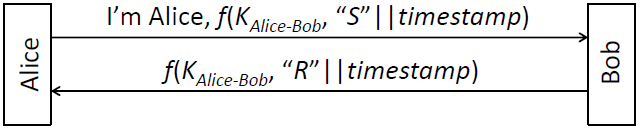
\includegraphics[height=4cm, width=12cm, keepaspectratio]{Immagini/autenticazione/ImgS56bis.png}}
	\caption{Mutua autenticazione basata sulla sincronizzazione degli orologi e su un segreto condiviso $K_{Alice-Bob}$}\label{fig:ImgS56bis} 	
\end{figure}
\subsection{Cifratura e integrità dei dati}
Al fine di fornire protezione dell'integrità e della confidenzialità dei dati da trasmettere dopo lo scambio di autenticazione, Alice e Bob devono necessariamente usare la crittografia (a chiave segreta) per cifrare e/o aggiungere dei controlli di integrità crittografici.\\
L'esecuzione di tali operazioni richiede preliminarmente che le parti stabiliscano una chiave segreta di sessione (session key) anche se già condividono dei segreti a lungo termine che permetterebbero di cifrare o di eseguire dei controlli di integrità.\\
Tipicamente, una chiave di sessione viene stabilita modificando lo scambio di autenticazione in modo tale che, terminato l'handshake, le due parti condividano una chiave segreta. Esamineremo come procedere in relazione ai seguenti scambi di autenticazione:
\begin{itemize}
\item Chiave segreta: Alice e Bob condividono una chiave segreta $K_{Alice-Bob}$ (che non e la chiave di sessione)
\item Chiave pubblica: Alice e Bob conoscono ciascuno la chiave pubblica dell'altro e chiaramente la propria chiave privata
\item Chiave pubblica unidirezionale: soltanto una parte ha una coppia $<PU,PR>$, quindi l'autenticazione è unidirezionale.
\end{itemize}
Ovviamente, un intercettatore non deve essere in grado di ottenere la chiave di sessione.
\subsubsection{Autenticazione a chiave segreta}
Sia $K_{Alice-Bob}$ il segreto a lungo termine condiviso tra Alice e Bob, si consideri lo schema di autenticazione riportato in \figurename ~\ref{fig:ImgS61bis} - anche se quanto detto potrà applicarsi al caso di mutua autenticazione (anziché $R$ ci saranno $R_{1}$ e $R_{2}$) e autenticazione mediante $timestamp$ anziché sfide random $R$ – c'è sufficiente informazione per stabilire una chiave di sessione condivisa.
\begin{figure}[htbp]
	\centering%
	\subfigure%
	{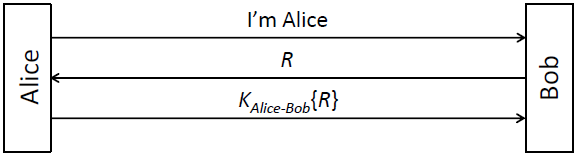
\includegraphics[height=4cm, width=12cm, keepaspectratio]{Immagini/autenticazione/ImgS61bis.png}}
	\caption{Autenticazione con chiave segreta $K_{Alice-Bob}$}\label{fig:ImgS61bis} 	
\end{figure}
Una possibile chiave di sessione è $K_{s} = (K_{Alice-Bob}+1)\lbrace R\rbrace$; in generale, una chiave di sessione può ottenersi modificando $K_{Alice-Bob}$ in qualche modo ($K_{modified} = f(K_{Alice-Bob})$) e cifrando la sfida $R$ con la chiave modificata: il risultato è la chiave di sessione $K_{modified} = K_{s} = (f(K_{Alice-Bob})\lbrace R\rbrace$\\
Si noti che $K_{Alice-Bob}\lbrace R\rbrace$ non può utilizzarsi come chiave di sessione perché è trasmessa
da Alice nel terzo messaggio dell'handshake.
Si noti anche che $K_{Alice-Bob}\lbrace R+1\rbrace$ non è sicura per una ragione molto sottile (\figurename ~\ref{fig:ImgS65bis}):
\begin{figure}[htbp]
	\centering%
	\subfigure%
	{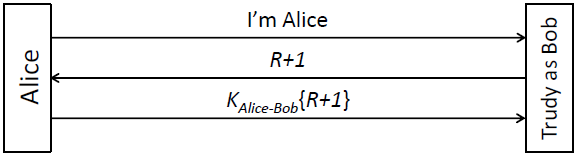
\includegraphics[height=4cm, width=12cm, keepaspectratio]{Immagini/autenticazione/ImgS65bis.png}}
	\caption{Trudy impersona Bob}\label{fig:ImgS65bis} 	
\end{figure}
Si supponga che Alice e Bob abbiano iniziato una conversazione e Bob abbia inviato $R$ come sfida; Trudy potrebbe aver registrato l'intera conversazione, cifrata con $K_{s} = K_{Alice-Bob}\lbrace R\rbrace$. In seguito, Trudy potrebbe impersonare l'indirizzo di rete di Bob in una successiva comunicazione con Alice e dichiarandosi Bob, potrebbe inviare $R+1$ come sfida, alla quale Alice risponderebbe con $K_{Alice-Bob}\lbrace R+1\rbrace$. A questo punto Trudy sarebbe in grado di decifrare la precedente conversazione (registrata) tra Alice e Bob.\\
In definitiva, Alice e Bob, dopo lo scambio di autenticazione, conoscono, oltre $K_{Alice-Bob}$, anche $R$: molte combinazioni di tali quantità permettono di ottenere una chiave di sessione sicura, ma ci sono anche combinazioni non accettabili, infatti si noti che una buona chiave di sessione deve variare da sessione a sessione, non essere indovinabile da un intercettatore e non deve ottenersi cifrando con $K_{Alice-Bob}$ una quantità $X$, dove $X$ è un valore che può essere predetto o estratto da un intruso (e.g. $X = R + 1$).
\subsubsection{Autenticazione a chiave pubblica}
Nel caso di autenticazione a chiave pubblica bidirezionale Alice e Bob conoscono la propria chiave privata e la chiave pubblica dell'altro. Per definire una chiave (segreta) di sessione condivisa $K_{s}$ esistono varie possibilità.\\ \\
Nello schema in \figurename ~\ref{fig:ImgS67bis} una parte, diciamo Alice, sceglie un numero random $R$ (che sarebbe la chiave di sessione), lo cifra con la chiave pubblica di Bob ed invia a Bob $\lbrace R\rbrace_{Bob}$.
\begin{figure}[htbp]
	\centering%
	\subfigure%
	{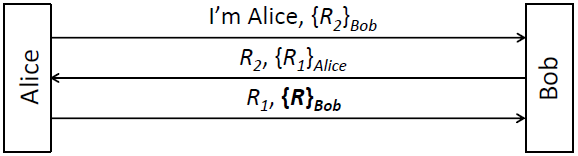
\includegraphics[height=4cm, width=12cm, keepaspectratio]{Immagini/autenticazione/ImgS67bis.png}}
	\caption{Autenticazione a chiave pubblica bidirezionale, $K_{s} = R$ e Alice invia $\lbrace R\rbrace_{Bob}$}\label{fig:ImgS67bis} 	
\end{figure}
Questo schema presenta la seguente vulnerabilità: un intruso, Trudy, può dirottare la conversazione scegliendo un suo $R$, cifrandolo con la chiave pubblica di Bob e inviando il risultato a Bob al posto della chiave cifrata fornita da Alice; contestualmente dovrebbe impersonare l'indirizzo di rete di Alice.\\ \\
In riferimento allo schema in \figurename ~\ref{fig:ImgS69bis}, rispetto a prima Alice firma la quantità $\lbrace R\rbrace_{Bob}$ e invia a Bob $[\lbrace R\rbrace_{Bob}]_{Alice}$; Bob verifica prima la firma di Alice usando $PU_{Alice}$ e poi decifra con la propria chiave privata $\lbrace R\rbrace_{Bob}$ riottenendo $R$.
\begin{figure}[htbp]
	\centering%
	\subfigure%
	{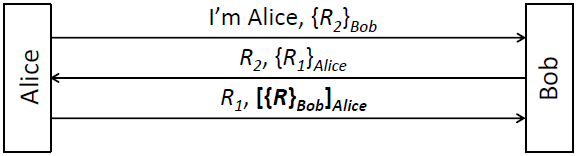
\includegraphics[height=4cm, width=12cm, keepaspectratio]{Immagini/autenticazione/ImgS69bis.png}}
	\caption{Autenticazione a chiave pubblica bidirezionale, $K_{s} = R$ e Alice invia $[\lbrace R\rbrace_{Bob}]_{Alice}$}\label{fig:ImgS69bis} 	
\end{figure}
L'attacco visto per il caso precedente (in cui Trudy sceglie un proprio $R$, in luogo di quello di Alice, e lo invia a Bob crittografato) ora non può funzionare perché Trudy non è in grado di forgiare la firma di Alice; tuttavia, se si vuole essere paranoici, c'è ancora una "piccola" vulnerabilità che può essere ridotta parzialmente (vedi caso (3)) o del tutto (vedi caso (4)). La vulnerabilità è la seguente:\\
si supponga che Trudy registri una intera conversazione tra Alice e Bob, inclusi i dati cifrati con la chiave di
sessione; si supponga inoltre che "successivamente" (dopo un minuto/giorno/mese) Trudy riesca a violare il server
Bob e ad ottenere tutti i suoi segreti (quindi anche $PR_{Bob}$); ottenendo $PR_{Bob}$ Trudy può recuperare la chiave di sessione dalle informazioni trasmesse: in particolare da $[\lbrace R\rbrace_{Bob}]_{Alice}$ può ottenere $K_{s} = R$. A questo punto Trudy può decifrare la conversazione cifrata tra Alice e Bob, precedentemente registrata.\\
In altri termini la soluzione (2) permette di sferrare degli attacchi alla confidenzialità "retroattivi" se nel futuro un avversario riuscisse a violare Bob.\\ \\
Nello schema in \figurename ~\ref{fig:ImgS74bis} Alice genera una quantità random $R$ e invia $\lbrace R\rbrace_{Bob}$ a Bob; Bob genera una quantità random $P$ e invia $\lbrace P\rbrace_{Alice}$ a Alice; terminata la conversazione Alice e Bob dimenticheranno $R$ e $P$.
\begin{figure}[htbp]
	\centering%
	\subfigure%
	{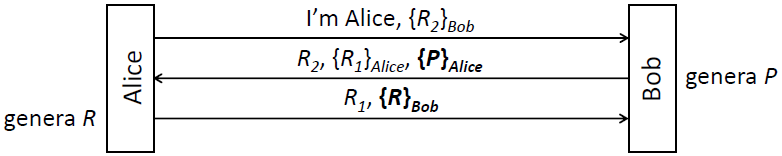
\includegraphics[height=4cm, width=12cm, keepaspectratio]{Immagini/autenticazione/ImgS74bis.png}}
	\caption{$K_{s} = R \oplus P$}\label{fig:ImgS74bis} 	
\end{figure}
Definendo $K_{s} = R \oplus P$, per ottenere la chiave di sessione, Trudy deve registrare lo scambio tra Alice e Bob,  violare Bob per ottenere $PR_{Bob}$ e quindi $R$, ma deve anche violare Alice per ottenere $PR_{Alice}$ e quindi $P$, (i.e. per ottenere $K_{s}$ Trudy dovrebbe violare entrambi).\\ \\
Alice e Bob possono effettuare uno scambio Diffie-Hellman autenticato (\figurename ~\ref{fig:ImgS77bis}), in cui ognuno firma la quantità da inviare all'altro (si supponga che le quantità $g$ e $p$ siano pubbliche).
\begin{figure}[htbp]
	\centering%
	\subfigure%
	{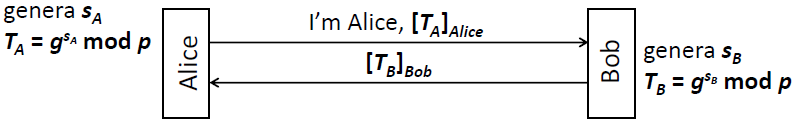
\includegraphics[height=4cm, width=12cm, keepaspectratio]{Immagini/autenticazione/ImgS77bis.png}}
	\caption{Autenticazione a chiave pubblica bidirezionale, uso di D-H con $K_{s} = K_{AB} = T_{B}^{s_{A}}modp = T_{A}^{s_{B}}modp = K_{BA}$}\label{fig:ImgS77bis} 	
\end{figure}
Usando Diffie-Hellman autenticato anche se Trudy riesce a violare sia Alice che Bob, ma non potrà comunque essere in grado di decifrare delle conversazioni registrate perché non è in grado di dedurre né $S_{A}$ né $S_{B}$.
\subsubsection{Autenticazione a chiave pubblica unidirezionale}
In alcuni casi solo una delle parti ha una coppia $<chiave-pubblica, chiave-privata>$, in particolare spesso, come nel caso di SSL, si assume che i server abbiano le chiavi pubbliche certificate, e che i client non si preoccupino
di ottenere chiavi e certificati, pertanto l'autenticazione crittografica è unidirezionale. In questi casi il protocollo assicura il client (Alice) che sta contattando il server Bob giusto, ma terminato la scambio di autenticazione, che permette tra l'altro di definire una chiave di sessione, il server non ha ancora autenticato il client. Quest'ultimo si autentica dopo lo scambio di autenticazione inviando username e password, cifrati con la
chiave di sessione $K_{s}$.\\ 
Vediamo ora due possibili modi per stabilire una chiave di sessione condivisa $K_{s}$ durante lo scambio di autenticazione a chiave pubblica unidirezionale.\\ \\
(a) \textbf{$K_{s} = R$ e Alice invia $\lbrace R\rbrace_{Bob}$} (\figurename ~\ref{fig:ImgS81bis}): 
\begin{figure}[htbp]
	\centering%
	\subfigure%
	{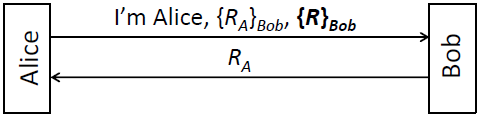
\includegraphics[height=4cm, width=12cm, keepaspectratio]{Immagini/autenticazione/ImgS81bis.png}}
	\caption{Autenticazione a chiave pubblica unidirezionale, $K_{s} = R$ e Alice invia $\lbrace R\rbrace_{Bob}$}\label{fig:ImgS81bis} 	
\end{figure}
Alice sceglie un numero random $R$, lo cifra con la chiave pubblica di Bob ed invia $\lbrace R\rbrace_{Bob}$. Si noti che tale schema presenta le debolezze viste nel caso (1), i.e. Trudy può registrare una intera conversazione e decifrarla; se riesce in futuro a violare Bob, Trudy può sostituire un suo $\lbrace R\rbrace_{Bob}$ e dirottare la
conversazione seguente. Tale debolezza è meno critica in un contesto dove non è necessaria una mutua autenticazione.\\\ \\
(b) Bob e Alice possono effettuare uno \textbf{scambio Diffie-Hellman}, dove Bob firma la sua quantità $T_{B}$ (\figurename ~\ref{fig:ImgS82bis})
\begin{figure}[htbp]
	\centering%
	\subfigure%
	{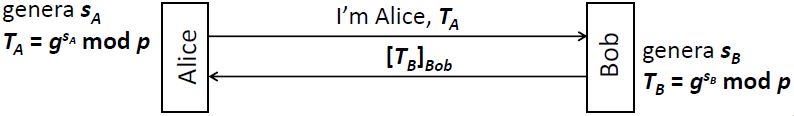
\includegraphics[height=4cm, width=12cm, keepaspectratio]{Immagini/autenticazione/ImgS82bis.png}}
	\caption{Autenticazione a chiave pubblica unidirezionale, uso di D-H con $K_{s} = K_{AB} = T_{B}^{s_{A}}modp = T_{A}^{s_{B}}modp = K_{BA}$}\label{fig:ImgS82bis} 	
\end{figure}
Si noti che Alice non può firmare nulla non disponendo di una coppia $<PU, PR>$. Si noti anche che il caso (b) rispetto al caso (a) è un po' più sicuro, infatti Trudy non può ottenere la chiave di sessione $K_{s}$ usata in
una precedente conversazione neanche violando Bob (si assuma che Bob dimentichi $K_{s}$ non appena la conversazione con Alice termina).\\ \\
Si noti che nessuno degli schemi (a) e (b) assicura a Bob di comunicare con la vera Alice,  ma in entrambi i casi Bob è sicuro che l'intera conversazione sia con una singola persona.
\subsubsection{Confidenzialità e integrità}
Tipicamente, la conversazione che segue lo scambio di autenticazione viene cifrata con la chiave di sessione per
proteggere la confidenzialità, inoltre viene applicato un controllo di integrità ai vari messaggi trasmessi (MIC o MAC), ottenuto con tecniche crittografiche a chiave segreta oppure sfruttando degli algoritmi di digest.\\
Si è visto che non esiste un algoritmo standard per proteggere contemporaneamente confidenzialità e integrità disponendo di una sola chiave (la chiave di sessione $K_{s}$) ed effettuando una singola operazione crittografica; pertanto si applicano alcune delle seguenti soluzioni che proteggono confidenzialità ed integrità in due fasi:
\begin{itemize}
\item stabilire due chiavi di sessione nello scambio di autenticazione $K_{sc}$ (chiave di sessione per la confidenzialità) e $K_{si}$ (chiave i sessione per l'integrità)
\item derivare una chiave dall'altra, cambiando alcuni bit in modo deterministico $K_{si} = f(K_{sc})$
\item usare una sola chiave $K_{s}$, ma algoritmi crittografici distinti (e.g. confidenzialità tramite AES/CBC e integrità tramite HMAC)
\item includere un checksum debole per l'integrità all'interno di un algoritmo robusto per la protezione della confidenzialità: una volta stabilità una (o più) chiave di sessione, la conversazione, generalmente, consiste nello scambio di messaggi singolarmente cifrati e dei relativi MAC, quindi ogni volta che una parte riceve un messaggio lo
decifra ed esegue il controllo di autenticità, poi, eventualmente, può proseguire la conversazione
\end{itemize}
\section{Autenticazione mediata (con KDC)}
Lo scambio riportato in \figurename ~\ref{fig:ImgS94bis} illustra in modo esemplificato il ruolo di mediazione del KDC: questo non sa se è realmente Alice l'utente che ha chiesto di comunicare con Bob, quindi Trudy potrebbe spacciarsi per Alice, ma poi non riuscirebbe ad ottenere $K_{AB}$ e non sarebbe in grado di decifrare il messaggio
$K_{Alice}\lbrace use K_{AB} for Bob\rbrace$; Trudy al massimo può indurre il KDC ad inviare ad Alice un messaggio da lei non richiesto.
\begin{figure}[htbp]
	\centering%
	\subfigure%
	{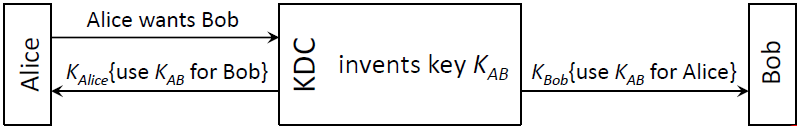
\includegraphics[height=4cm, width=12cm, keepaspectratio]{Immagini/autenticazione/ImgS94bis.png}}
	\caption{Operazioni svolte dal KDC (in linea di principio)}\label{fig:ImgS94bis} 	
\end{figure}
Le uniche parti che conoscono $K_{AB}$ dopo questo scambio sono Alice, Bob e il KDC, pertanto, dopo lo scambio Alice e Bob possono autenticarsi reciprocamente utilizzando il segreto condiviso $K_{AB}$. \\
Il protocollo precedente però non è quello utilizzato nella pratica, poiché se Alice invia immediatamente un messaggio a Bob, per i ritardi nella rete, è possibile che questo arrivi prima del messaggio che il KDC ha inviato a Bob; inoltre, il fatto che un utente qualsiasi, senza autenticarsi presso il KDC, possa indurre quest'ultimo ad aprire connessioni verso un suo qualsiasi utente comporta una serie di pericoli che dovrebbero essere gestiti (i.e. siccome è Alice che desidera comunicare con Bob la cosa più ragionevole, è che il KDC fornisca ad Alice tutte le informazioni che egli avrebbe fornito a Bob per instaurare una connessione sicura con Alice; e.g. nel protocollo Kerberos, l'informazione cifrata che il KDC invia ad Alice da passare a Bob è detta ticket per Bob).
\subsubsection{(P12) Protocollo 12 - Mediazione del KDC}
Nella pratica la mediazione del KDC avviene in modo simile a come illustrato in \figurename ~\ref{fig:ImgS97bis}
\begin{figure}[htbp]
	\centering%
	\subfigure%
	{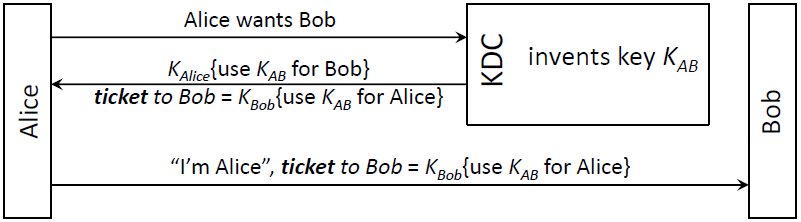
\includegraphics[height=4cm, width=12cm, keepaspectratio]{Immagini/autenticazione/ImgS97bis.png}}
	\caption{Operazioni svolte dal KDC (nella pratica)}\label{fig:ImgS97bis} 	
\end{figure}
Naturalmente Alice e Bob devono poi autenticarsi reciprocamente con una delle tecniche esaminate prima, i.e. ciascuno deve dimostrare all'altro di conoscere realmente $K_{AB}$.\\ \\
Il protocollo (P12) presenta la seguente vulnerabilità, anche se in pratica è improbabile che possa essere sfruttata da un attaccante: \\
si supponga che Trudy abbia rubato una vecchia chiave di Bob $K'_{Bob}$ (Bob scoprendolo potrebbe già aver provveduto a cambiarla) e che abbia anche rubato un vecchio messaggio di risposta del KDC ad Alice quando la chiave di Bob era ancora $K'_{Bob}$. Trudy attende che Alice richieda al KDC di parlare con Bob, poi sostituisce la risposta del KDC con quella vecchia in suo possesso, che appare ad Alice come una risposta ordinaria. Trudy può pertanto impersonare Bob, riesce a decifrare il ticket e ad ottenere la chiave di sessione.\\
Questa vulnerabilità, prevalentemente teorica, può essere rimossa non permettendo a Trudy di riusare (\textbf{reply}) vecchie risposte del KDC (e.g. aggiungendo un nounce $N_{1}$ alla richiesta iniziale di Alice e chiedendo al KDC di cifrarlo insieme alla chiave $K_{AB}$).\\
In \figurename ~\ref{fig:ImgS103bis} è rappresentato il protocollo (P12.1), ottenuto rimuovendo la vulnerabilità appena illustrata:
\begin{figure}[htbp]
	\centering%
	\subfigure%
	{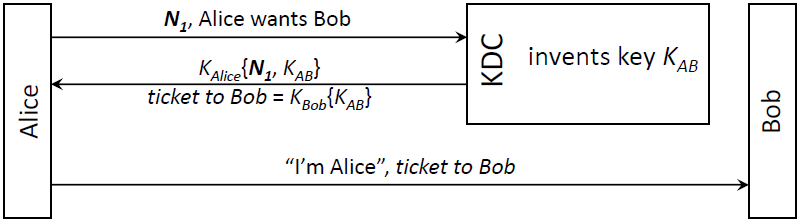
\includegraphics[height=4cm, width=12cm, keepaspectratio]{Immagini/autenticazione/ImgS103bis.png}}
	\caption{Protocollo (P12.1)}\label{fig:ImgS103bis} 	
\end{figure}
Nel protocollo (P12.1) sussiste ancora la seguente vulnerabilità:\\
si supponga che Trudy, utente del KDC, riesca a modificare la richiesta di Alice, sostituendo $"Bob"$ con $"Trudy"$. Il KDC restituirebbe ad Alice una chiave condivisa con Trudy e non con Bob (i.e. $K_{AT}$ e non $K_{AB}$), tuttavia, dalle informazioni ricevute, Alice non può rendersi conto di tale attacco (i.e. Alice è convinta di aver ricevuto $K_{AB}$), quindi Trudy potrebbe impersonare Bob senza che Alice se ne accorga.\\ \\
Il precedente attacco è sventabile aggiungendo alle informazioni che il KDC deve inviare ad Alice (cifrate con $K_{Alice}$) il destinatario della richiesta di connessione che ha ricevuto il KDC: in tal modo Alice può verificare se coincide con quello presente nella sua richiesta. Inoltre il KDC può aggiungere il nome dell'utente che ha effettuato la richiesta tra le informazioni che costituiscono il ticket per Bob (il motivo di tale scelta sarà chiaro più tardi).
Implementando le precedenti modifiche si ottiene il protocollo (P12.2), riportato in \figurename ~\ref{fig:ImgS106bis}
\begin{figure}[htbp]
	\centering%
	\subfigure%
	{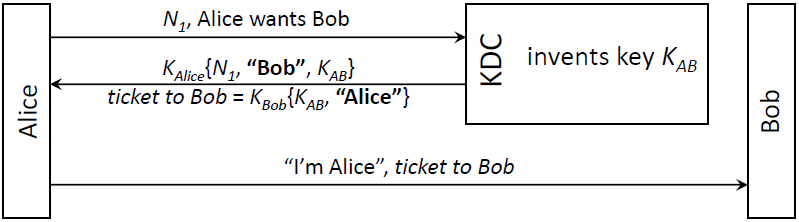
\includegraphics[height=4cm, width=12cm, keepaspectratio]{Immagini/autenticazione/ImgS106bis.png}}
	\caption{Protocollo (P12.2)}\label{fig:ImgS106bis} 	
\end{figure}
Il protocollo (P12.2), analogamente ai precedenti, non include uno scambio che permetta di autenticare reciprocamente Alice e Bob: per l'autenticazione reciproca ciascuno deve provare all'altro di conoscere $K_{AB}$. Alice sa che soltanto chi conosce $K_{Bob}$ può decifrare il ticket per Bob e quindi riottenere $K_{AB}$; Bob decifrando il ticket, oltre a $K_{AB}$, ottiene $"Alice"$ e sa pertanto che il KDC è stato contattato da Alice e che solo lui,
Alice e il KDC conoscono $K_{AB}$ (ciò spiega una delle modifiche inserite nel protocollo (P12.2)).\\
A questo punto Alice e Bob possono autenticarsi reciprocamente nel seguente modo:
\begin{itemize}
\item Alice, insieme al ticket, invia a Bob una sfida ($N_{2}$) cifrata con la chiave $K_{AB}$
\item Bob decifra il ticket e ottiene $K_{AB}$, quindi usa $K_{AB}$ per estrarre $N_{2}$, poi invia ad Alice $K_{AB}\lbrace N_{2}-1, N_{3}\rbrace$ ($N_{2}-1$ serve a provare ad Alice che conosce $K_{AB}$, $N_{3}$ è invece la sfida per Alice
\item Alice dimostra a Bob di conoscere $K_{AB}$ rispondendo alla sua sfida con $K_{AB}\lbrace N_{3}\rbrace$
\end{itemize}
Il protocollo (P12.3), riportato in \figurename ~\ref{fig:ImgS109bis}, include anche lo scambio per autenticare reciprocamente Alice e Bob:
\begin{figure}[htbp]
	\centering%
	\subfigure%
	{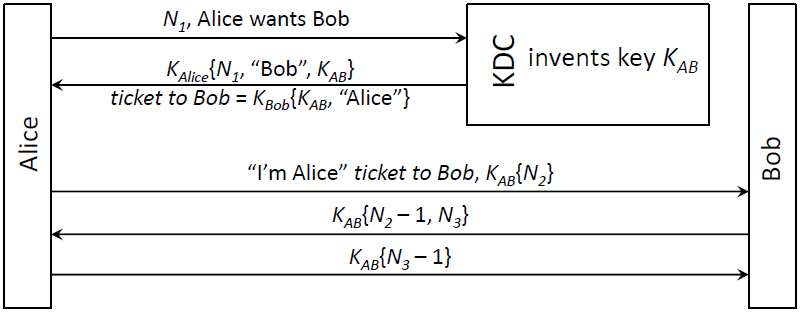
\includegraphics[height=4cm, width=12cm, keepaspectratio]{Immagini/autenticazione/ImgS109bis.png}}
	\caption{Protocollo (P12.3)}\label{fig:ImgS109bis} 	
\end{figure}
\subsubsection{Protocollo di Needham-Schroeder}
Il protocollo di Needham-Schroeder (\figurename ~\ref{fig:ImgS111bis}) in pratica coincide con il protocollo (P12.3),  tranne per il fatto che il KDC include il ticket per Bob tra le informazioni da cifrare con $K_{Alice}$. Si osservi che ciò non migliora la sicurezza, in quanto il ticket per Bob è qualcosa di indecifrabile per Alice (tale ulteriore cifratura poteva pertanto omettersi).
\begin{figure}[htbp]
	\centering%
	\subfigure%
	{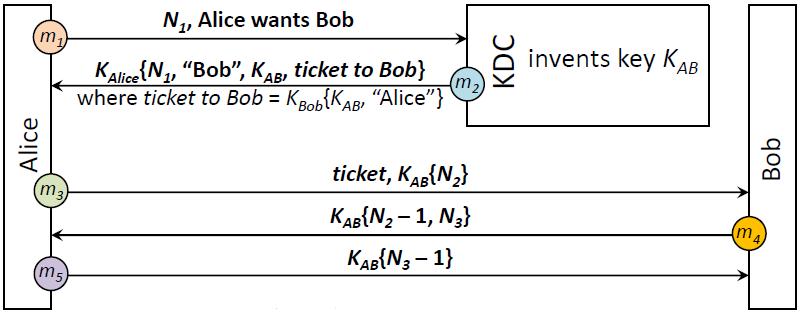
\includegraphics[height=4cm, width=12cm, keepaspectratio]{Immagini/autenticazione/ImgS111bis.png}}
	\caption{Protocollo di Needham-Schroeder}\label{fig:ImgS111bis} 	
\end{figure}




